\hypertarget{ux9065ux63a7ux5c0fux8f66}{%
\subsection{遥控小车}\label{ux9065ux63a7ux5c0fux8f66}}

使用 EV3 主机上的按键控制小车还是比较麻烦,能不能通过遥控来控制小车呢?

当然可以!

乐高提供了一个红外线传感器和遥控器:

 
 \begin{figure}[htp]
	\centering
	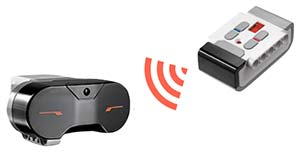
\includegraphics[width=0.6\linewidth]{fig/1346303361548354l.png}
\end{figure}


但是红外遥控器需要很强的方向性,而且那个遥控器太简陋了,连个摇杆都没有。

还有一种方式是使用蓝牙手柄,这样我们就可以找一个游戏手柄直接通过蓝牙控制小车,太方便了有木有!

我找了一个任天堂的游戏手柄:

 
 \begin{figure}[htp]
	\centering
	
\includegraphics[width=0.6\linewidth]{fig/1346304282198081l.png}
\end{figure}


理论上支持蓝牙的游戏手柄都是可用的,标准游戏手柄按键如下:

\begin{pythoncode}
   ┌──────┐                   ┌──────┐
  ┌┴─────┐│                  ┌┴─────┐│
┌─┴──────┴┴──────────────────┴──────┴┴─┐
│               ┌─┐ ┌─┐         ┌─┐    │
│   ┌─┐         └─┘ └─┘      ┌─┐│X│    │
│ ┌─┘ └─┐        -   +       │Y│└─┘┌─┐ │
│ └─┐ ┌─┘       ┌─┐ ┌─┐      └─┘┌─┐│A│ │
│   └─┘         └─┘ └─┘         │B│└─┘ │
│         ┌─┐    S   H    ┌─┐   └─┘    │
│       ┌─┘ └─┐         ┌─┘ └─┐        │
│       └─┐ ┌─┘         └─┐ ┌─┘        │
│         └─┘             └─┘          │
│       ────────────────────────       │
│      /                        \      │
│     /                          \     │
└────/                            \────┘
\end{pythoncode}

把游戏手柄和 EV3 主机用蓝牙连起来很简单,但是怎么用 Python
程序读取手柄的输入?

一般来说,从外部设备读取输入时,应用程序并不直接与外设打交道,而是由操作系统通过驱动程序连接外设,然后,通过操作系统提供的
API 读取输入。Windows 程序可以通过 DirectX 访问外设,运行在网页的
JavaScript 程序可以通过浏览器提供的 Gamepad API。

EV3 主机运行的是 Debian Linux,那么 Python 程序如何在 Linux
下读取手柄的输入?

在 Linux
中,系统把每个外设都映射为文件,每个设备的输入也被映射为文件。\texttt{/proc}目录挂载的就是
Linux 的虚拟文件系统,映射 Linux 的进程信息和设备信息。我们登录到
EV3,查看\texttt{/proc/bus/input/devices}文件:

\begin{pythoncode}
$ cat /proc/bus/input/devices 
I: Bus=0000 Vendor=0000 Product=0000 Version=0000
N: 
P: Phys=
S: Sysfs=/devices/platform/sound/input/input0
U: Uniq=
H: Handlers=kbd event0 
B: PROP=0
B: EV=40001
B: SND=6

I: Bus=0019 Vendor=0001 Product=0001 Version=0100
N: 
P: Phys=gpio-keys/input0
S: Sysfs=/devices/platform/gpio_keys/input/input1
U: Uniq=
H: Handlers=kbd event1 
B: PROP=0
B: EV=3
B: KEY=1680 0 0 10004000
\end{pythoncode}

这个文件列出了目前系统可用的输入设备,上述两段分别代表扬声器和按钮设备。如果我们把蓝牙手柄连接到
EV3,再查看文件,发现多了一段内容:

\begin{pythoncode}
I: Bus=0005 Vendor=057e Product=2009 Version=0001
N: 
P: Phys=00:17:ec:13:d8:1d
S: Sysfs=/devices/platform/soc@1c00000/serial8250.2/tty/ttyS2/hci0/hci0:2/0005:057E:2009.0003/input/input4
U: Uniq=00:90:e3:9b:ec:e9
H: Handlers=event2 
B: PROP=0
B: EV=10001b
B: KEY=ffff0000 0 0 0 0 0 0 0 0 0
B: ABS=3001b
B: MSC=10
\end{pythoncode}

我们通过\texttt{N:}
来搜索手柄设备,然后,通过\texttt{H:\ Handlers=xxx}获取设备的输入文件。例如,上述蓝牙手柄的名称是\texttt{Pro\ Controller},输入是\texttt{event2},对应到系统文件就是\texttt{/dev/input/event2}。Python
代码实现如下:

定义\texttt{InputDevice}类表示输入设备:

\begin{pythoncode}
class InputDevice():
    def __init__(self):
        self.name = ''
        self.handler = ''

    def __str__(self):
        return '<Input Device: name=%s, handler=%s>' % (self.name, self.handler)

    def setName(self, name):
        if len(name) >= 2 and name.startswith('"') and name.endswith('"'):
            name = name[1:len(name)-1]
        self.name = name

    def setHandler(self, handlers):
        for handler in handlers.split(' '):
            if handler.startswith('event'):
                self.handler = handler
\end{pythoncode}

定义函数\texttt{listDevices()}通过读取\texttt{/proc/bus/input/devices}文件获取所有设备:

\begin{pythoncode}
def listDevices():
    devices = []
    with open('/proc/bus/input/devices', 'r') as f:
        device = None
        while True:
            s = f.readline()
            if s == '':
                break
            s = s.strip()
            if s == '':
                devices.append(device)
                device = None
            else:
                if device is None:
                    device = InputDevice()
                if s.startswith('N: Name='):
                    device.setName(s[8:])
                elif s.startswith('H: Handlers='):
                    device.setHandler(s[12:])
    return devices
\end{pythoncode}

定义函数\texttt{detectJoystick()}通过名字模糊查找手柄设备:

\begin{pythoncode}
def detectJoystick(joystickNames):
    for device in listDevices():
        for joystickName in joystickNames:
            if joystickName in device.name:
                
                return '/dev/input/%s' % device.handler
    
    return None
\end{pythoncode}

搜索到手柄设备后打开文件读取输入:

\begin{pythoncode}
eventFile = detectJoystick(['Controller'])
if eventFile:
    with open(eventFile, 'rb') as infile:
        while True:
            
\end{pythoncode}

现在最关键的问题来了:\texttt{eventX}文件应该以何种格式读取?

让我们搜索一下 Linux 文档,在
\href{https://www.kernel.org/doc/Documentation/input/input.txt}{input.txt}
中详细说明了\texttt{eventX}文件的输入格式。Linux
系统把每一个输入事件都封装为一个 C 结构体让我们直接读取:

\begin{pythoncode}
struct input_event {
    struct timeval time; 
    unsigned short type; 
    unsigned short code; 
    unsigned int value; 
};
\end{pythoncode}

每次读取 24 字节并按照 C
的\texttt{struct}类型解码,即可得到手柄输入的全部信息。在 Python
程序中,可以用\texttt{struct}读取:

\begin{pythoncode}
FORMAT = 'llHHI'
EVENT_SIZE = struct.calcsize(FORMAT)
with open(eventFile, 'rb') as infile:
    while True:
        event = infile.read(EVENT_SIZE)
        _, _, t, c, v = struct.unpack(FORMAT, event)
        print('t = %s, c = %s, v = %s' % (t, c, v))
\end{pythoncode}

注意到\texttt{unpack()}方法的返回值,我们丢弃了前两个 8
字节整数,保留了\texttt{t}、\texttt{c}、\texttt{v},分别是 2
字节无符号整数、2 字节无符号整数和 4 字节无符号整数。

根据 Linux
文档,再打印出每个事件的详细数据,把手柄的按键和摇杆都按一遍,就可以得到按键编码如下:

\texttt{t==1}时表示按键,此时\texttt{v==1}表示按下,\texttt{v==0}表示释放,\texttt{v==2}表示持续按下,对应的\texttt{c}表示按键编码。要检测\texttt{A}、\texttt{B}按钮按下,可以这么写:

\begin{pythoncode}
if t == 1 and v == 1:
    if c == 305:
        
        pass
    if c == 304:
        
        pass
\end{pythoncode}

摇杆数据则比较复杂,类型\texttt{t==3}表示摇杆,如果\texttt{c==0},表示左摇杆的左右移动,如果\texttt{c==1},表示左摇杆的上下移动,\texttt{v}的值介于\texttt{0}\textasciitilde{}\texttt{65535},\texttt{32768}表示中心值,越往两侧偏移越多则越接近最大和最小值:

\begin{pythoncode}
      0
      ▲
      │
0 <───┼───> 65535
      │
      ▼
    65535
\end{pythoncode}

现在我们就可以通过一个读取手柄的无限循环来控制小车:

\begin{pythoncode}
def joystickLoop(robot, eventFile):
    FORMAT = 'llHHI'
    EVENT_SIZE = struct.calcsize(FORMAT)
    with open(eventFile, 'rb') as infile:
        while True:
            event = infile.read(EVENT_SIZE)
            _, _, t, c, v = struct.unpack(FORMAT, event)
            if t == 1 and v == 1:
                if c == 305:
                    
                    robot.setSpeed(1)
                elif c == 304:
                    
                    robot.setSpeed(-1)
                elif c == 307:
                    
                    return robot.inactive()
            elif t == 3:
                if c == 1:
                    
                    speed = 0
                    if v < 32768:
                        
                        speed = 1
                    elif v > 32768:
                        
                        speed = -1
                    robot.setSpeed(speed)
\end{pythoncode}

但是另一个问题来了:主线程通过死循环读取手柄输入,那么怎么读取超声波传感器的数据?

可以利用 Python
的\texttt{threading}启动多线程,在另一个线程中不断检测超声波传感器,并在条件达到的时候自动停车:

\begin{pythoncode}
def autoStopLoop(robot):
    while robot.active:
        if robot.speed > 0 and robot.ultrasonic.distance() < 200:
            robot.setSpeed(0)
        wait(100)

joystickEvent = detectJoystick(['Controller'])
robot = Robot()
t = threading.Thread(target=autoStopLoop, args=(robot,))
t.start()
joystickLoop(robot, joystickEvent)
\end{pythoncode}

到此为止,一个蓝牙手柄控制的机器人程序就宣告完成。试试效果:

\hypertarget{ux53c2ux8003ux6e90ux7801}{%
\subsubsection{参考源码}\label{ux53c2ux8003ux6e90ux7801}}

\href{https://github.com/michaelliao/learn-python3/tree/master/samples/micropython/rccar}{rccar}

